\documentclass[11pt,
			   %10pt, 
               %hyperref={colorlinks},
               aspectratio=43,
               hyperref={colorlinks}
               ]{beamer}
\usetheme{Singapore}
\usecolortheme[snowy, cautious]{owl}

\usepackage[utf8]{inputenc}
\usepackage[T1]{fontenc}
\usepackage[american]{babel}
\usepackage{graphicx}
\usepackage{hyperref}
\hypersetup{
    colorlinks=true,
    urlcolor=[rgb]{1,0,1},
    linkcolor=[rgb]{1,0,1}}
\definecolor{magenta}{RGB}{255, 0, 255}

\usepackage[natbib=true,style=numeric,backend=bibtex,useprefix=true]{biblatex}

\definecolor{OwlGreen}{RGB}{75,0,130} % easier to see
\setbeamertemplate{bibliography item}{\insertbiblabel}
\setbeamerfont{caption}{size=\footnotesize}
\setbeamertemplate{frametitle continuation}{}

\setcounter{tocdepth}{1}
\renewcommand*{\bibfont}{\scriptsize}
\addbibresource{bibliography.bib}

\renewcommand*{\thefootnote}{\fnsymbol{footnote}}

\usenavigationsymbolstemplate{}
\setbeamertemplate{footline}{%
    \raisebox{5pt}{\makebox{\hfill\makebox[20pt]{\color{gray}
          \scriptsize\insertframenumber}}}\hspace*{5pt}}

\author{\copyright\hspace{1pt}Patrick Hall\footnote{\tiny{This material is shared under a \href{https://creativecommons.org/licenses/by/4.0/deed.ast}{CC By 4.0 license} which allows for editing and redistribution, even for commercial purposes. However, any derivative work should attribute the author and H2O.ai.}}}
\title{Increasing Trust and Understanding in Machine Learning with Model Debugging }
\logo{
\includegraphics[height=8pt]{img/h2o_logo.png}}
\institute{\href{https://www.h2o.ai}{H\textsubscript{2}O.ai}}
\date{\today}
\subject{}

\begin{document}
	
	\maketitle
	
	\begin{frame}
	
		\frametitle{Contents}
		
		\tableofcontents{}
		
	\end{frame}

%-------------------------------------------------------------------------------
	\section{What?}
%-------------------------------------------------------------------------------

	\begin{frame}
		
		\frametitle{What is Model Debugging?}
		
		\begin{itemize}
			\item Model debugging is an emergent discipline focused on discovering and remediating errors in the internal mechanisms and outputs of machine learning models. 
			\item Model debugging attempts to test machine learning models like code (because the models are code).
			\item Model debugging promotes trust directly and enhances interpretability as a side-effect.
		\end{itemize}	
		
	\end{frame}

%-------------------------------------------------------------------------------
	\section{Why?}
%-------------------------------------------------------------------------------

	\begin{frame}
		
		\frametitle{Why Bother With Model Debugging?}
		
			\footnotesize{Machine learning models can be \textbf{inaccurate}.}
			\begin{columns}
				
				\column{0.5\linewidth}
				\centering
				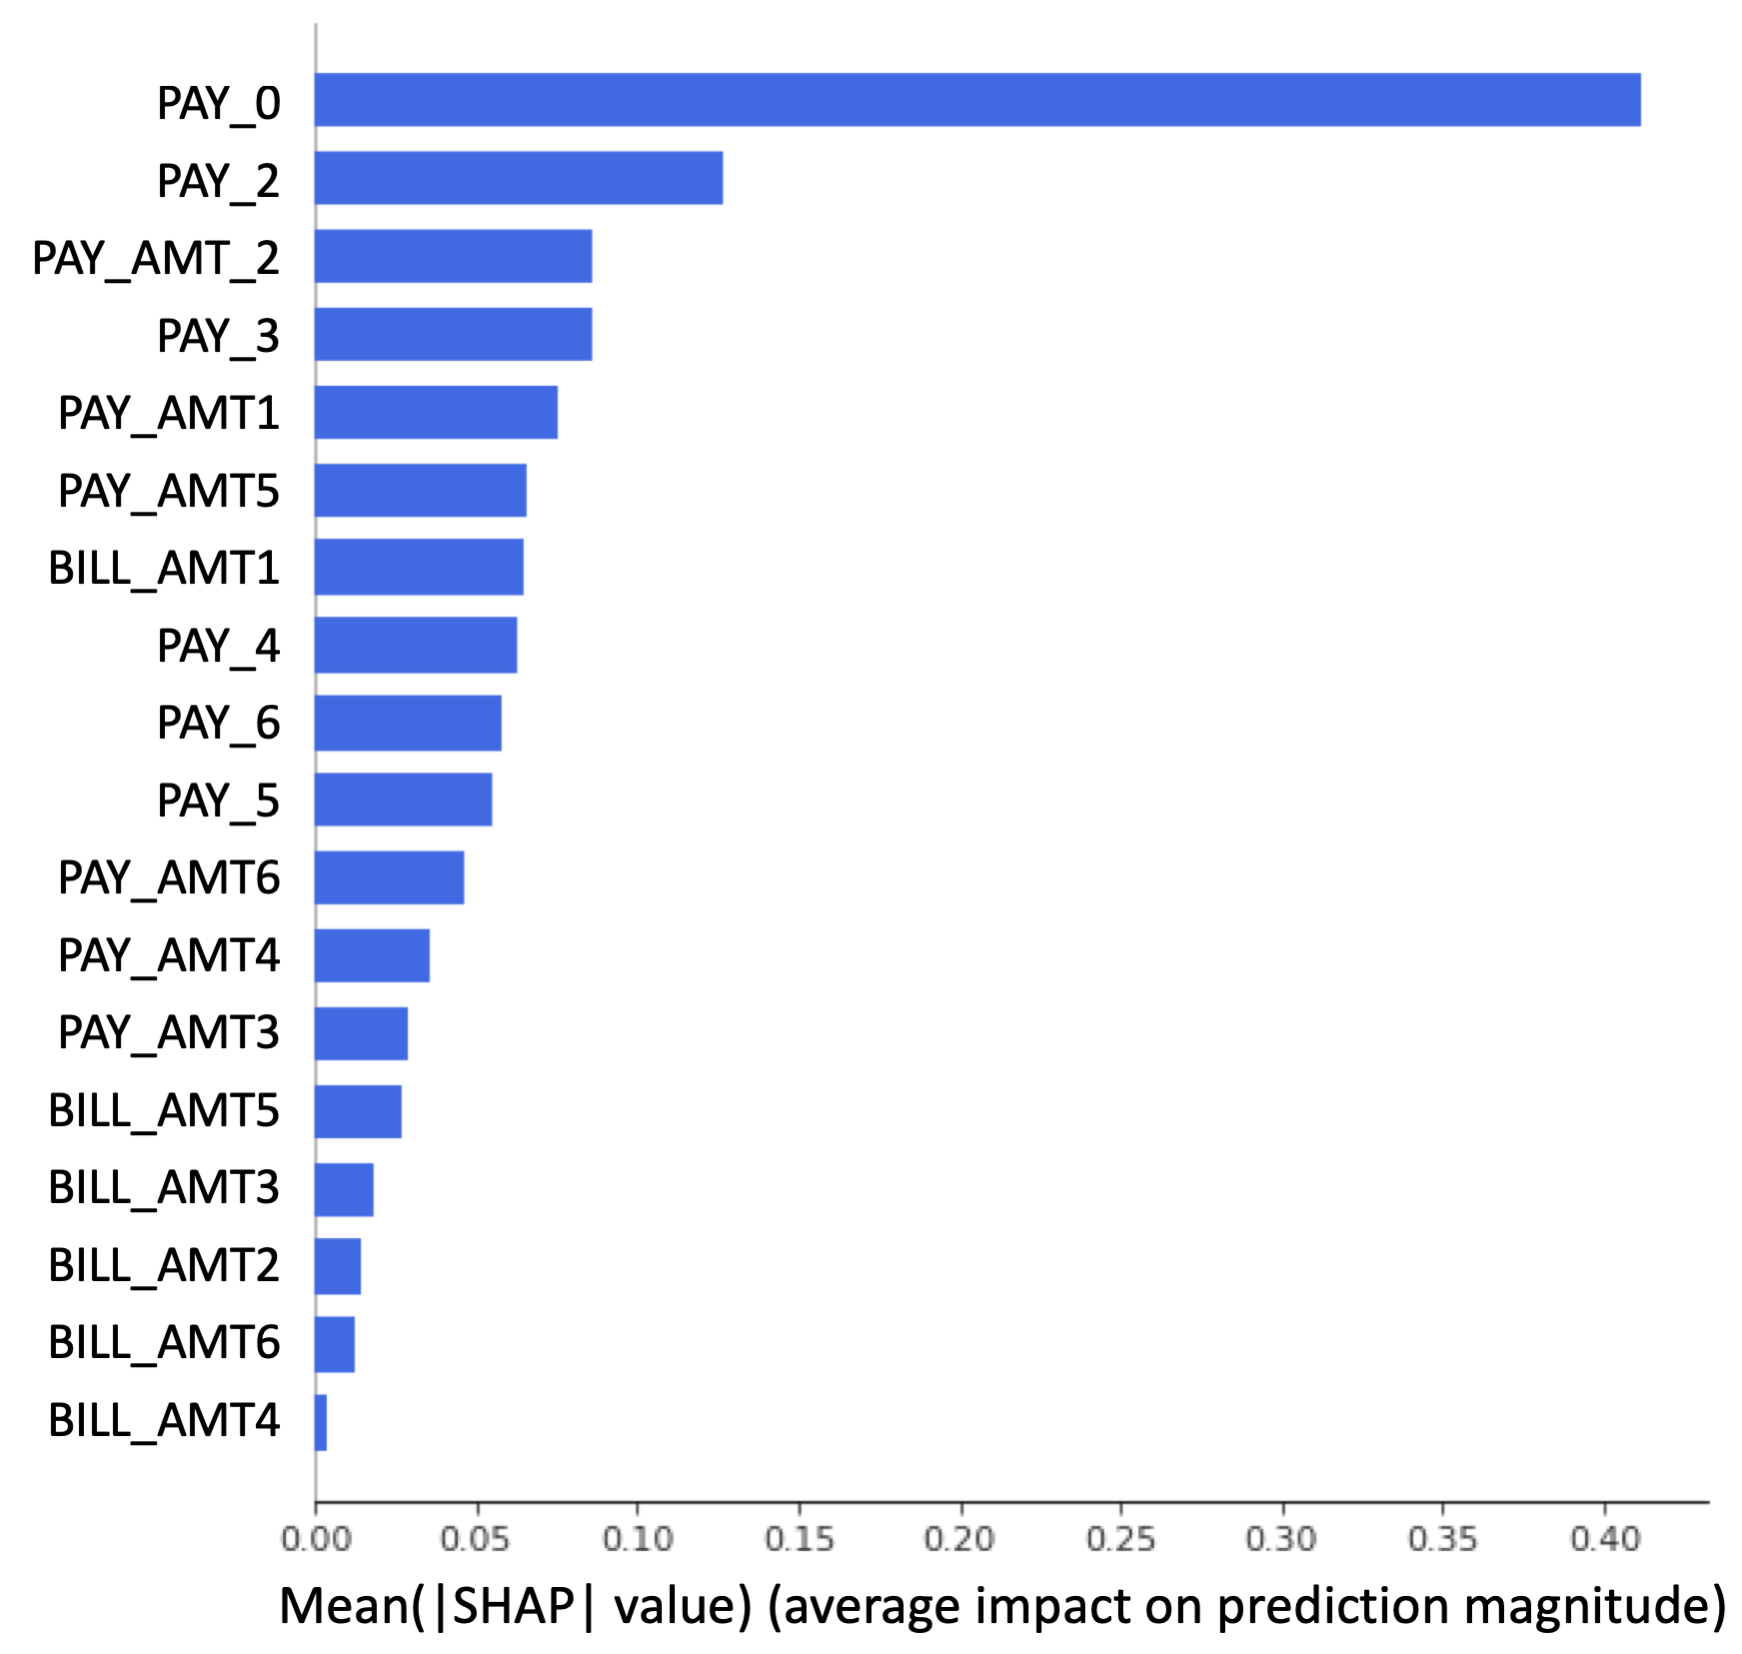
\includegraphics[height=125pt]{img/global_shap.png}\\
				\vspace{5pt}
				\tiny{This probability of default classifier, $g_{\text{mono}}$, over-emphasizes the most important feature, a customer's most recent repayment status, $\text{PAY\_0}$.}
				
				\column{0.5\linewidth}
				\centering
				\vspace{9pt}
				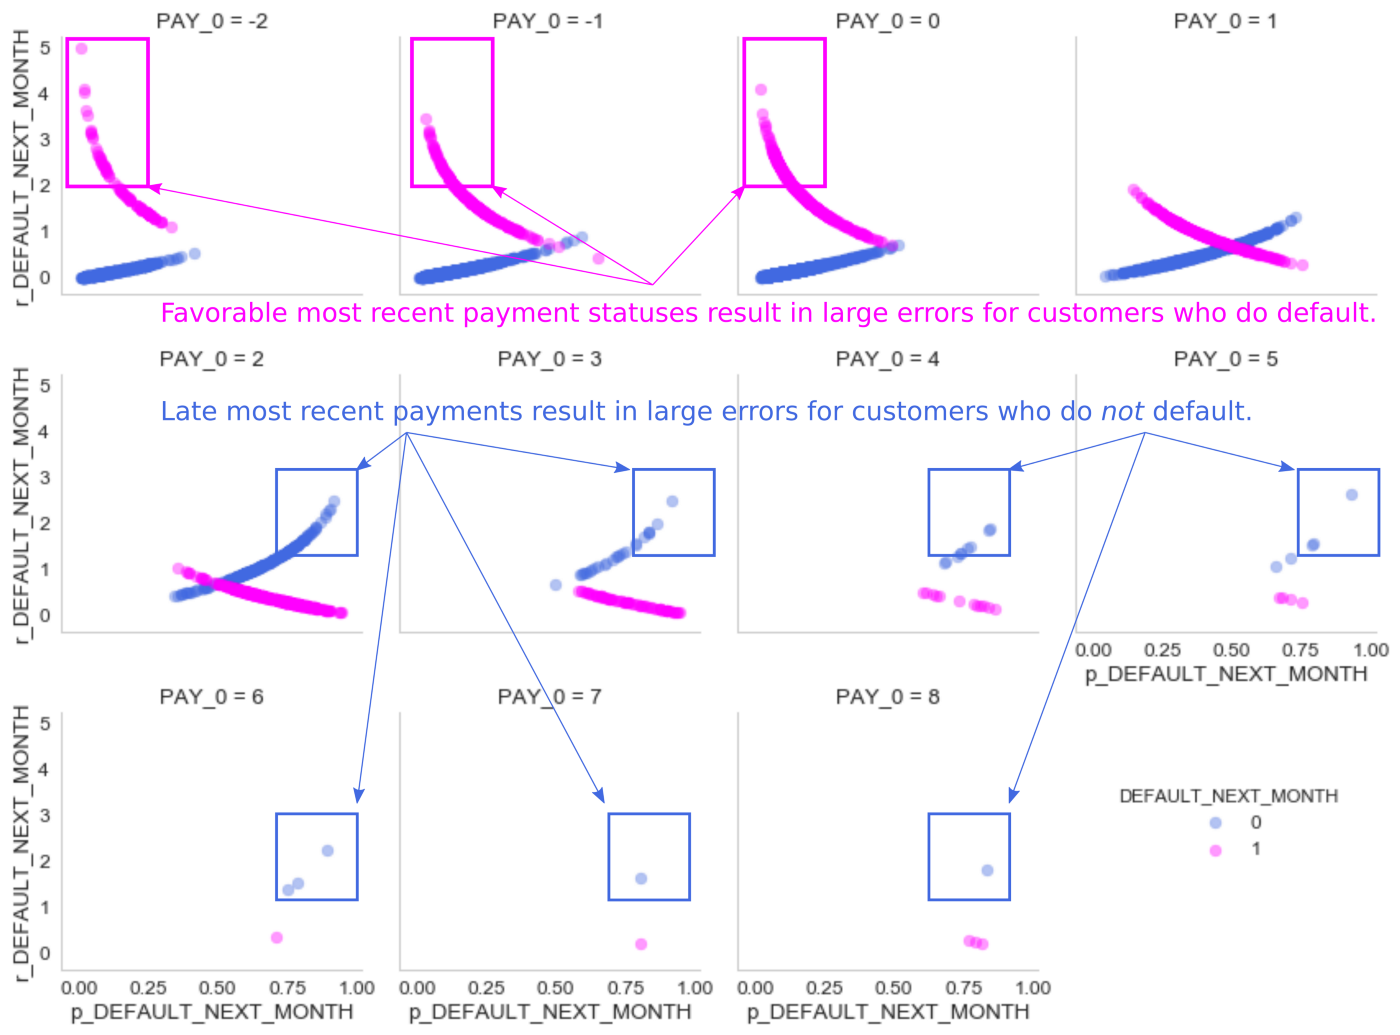
\includegraphics[height=120pt]{img/resid.png}\\
				\vspace{8pt}
				\tiny{$g_{\text{mono}}$ also struggles to predict default for favorable statuses, $-2  \leq \texttt{PAY\_0}  < 2$, and often cannot predict on-time payment when recent payments are late, $\text{PAY\_0} \geq 2$}.
				
			\end{columns}
			\normalsize
			
	\end{frame}
	
	\begin{frame}
		
		\frametitle{Why Bother With Model Debugging?}
		
		\footnotesize{Machine learning models can exhibit \textbf{disparate impact} or other types of\\sociological bias.}
		\vspace{10pt}	
		\begin{table}[htb!]
			\centering
			\footnotesize
			\begin{tabular}{ | p{1.2cm} | p{1.1cm} | p{1.3cm} | p{1.2cm}| p{1.2cm} | p{1.2cm} | p{1.2cm} | p{1.2cm} | }
				\hline
				& Adverse\newline Impact\newline Ratio & Accuracy Disparity & TPR\newline Disparity & TNR\newline Disparity & FPR\newline Disparity & FNR\newline Disparity \\ 
				\hline
				\texttt{single} & 0.89 & 1.03 & 0.99 & 1.03 & 0.85 & 1.01 \\
				\hline	
				\texttt{divorced} & 1.01 & 0.93 & 0.81 & 0.96 & \textcolor{magenta}{1.25} & 1.22 \\
				\hline
				\texttt{other} & \textcolor{magenta}{0.26} & 1.12 & \textcolor{magenta}{0.62} & 1.17 & \textcolor{magenta}{0} & \textcolor{magenta}{1.44} \\
				\hline	
			\end{tabular}
		\end{table}
		\footnotesize{Group disparity metrics are out-of-range for $g_{\text{mono}}$ across different marital statuses.}
		\normalsize
		
	\end{frame}
	
	\begin{frame}
		
		\frametitle{Why Bother With Model Debugging?}
		
		\footnotesize{Machine learning models can have \textbf{security vulnerabilities}}.
		\begin{figure}[htb]
			\begin{center}
				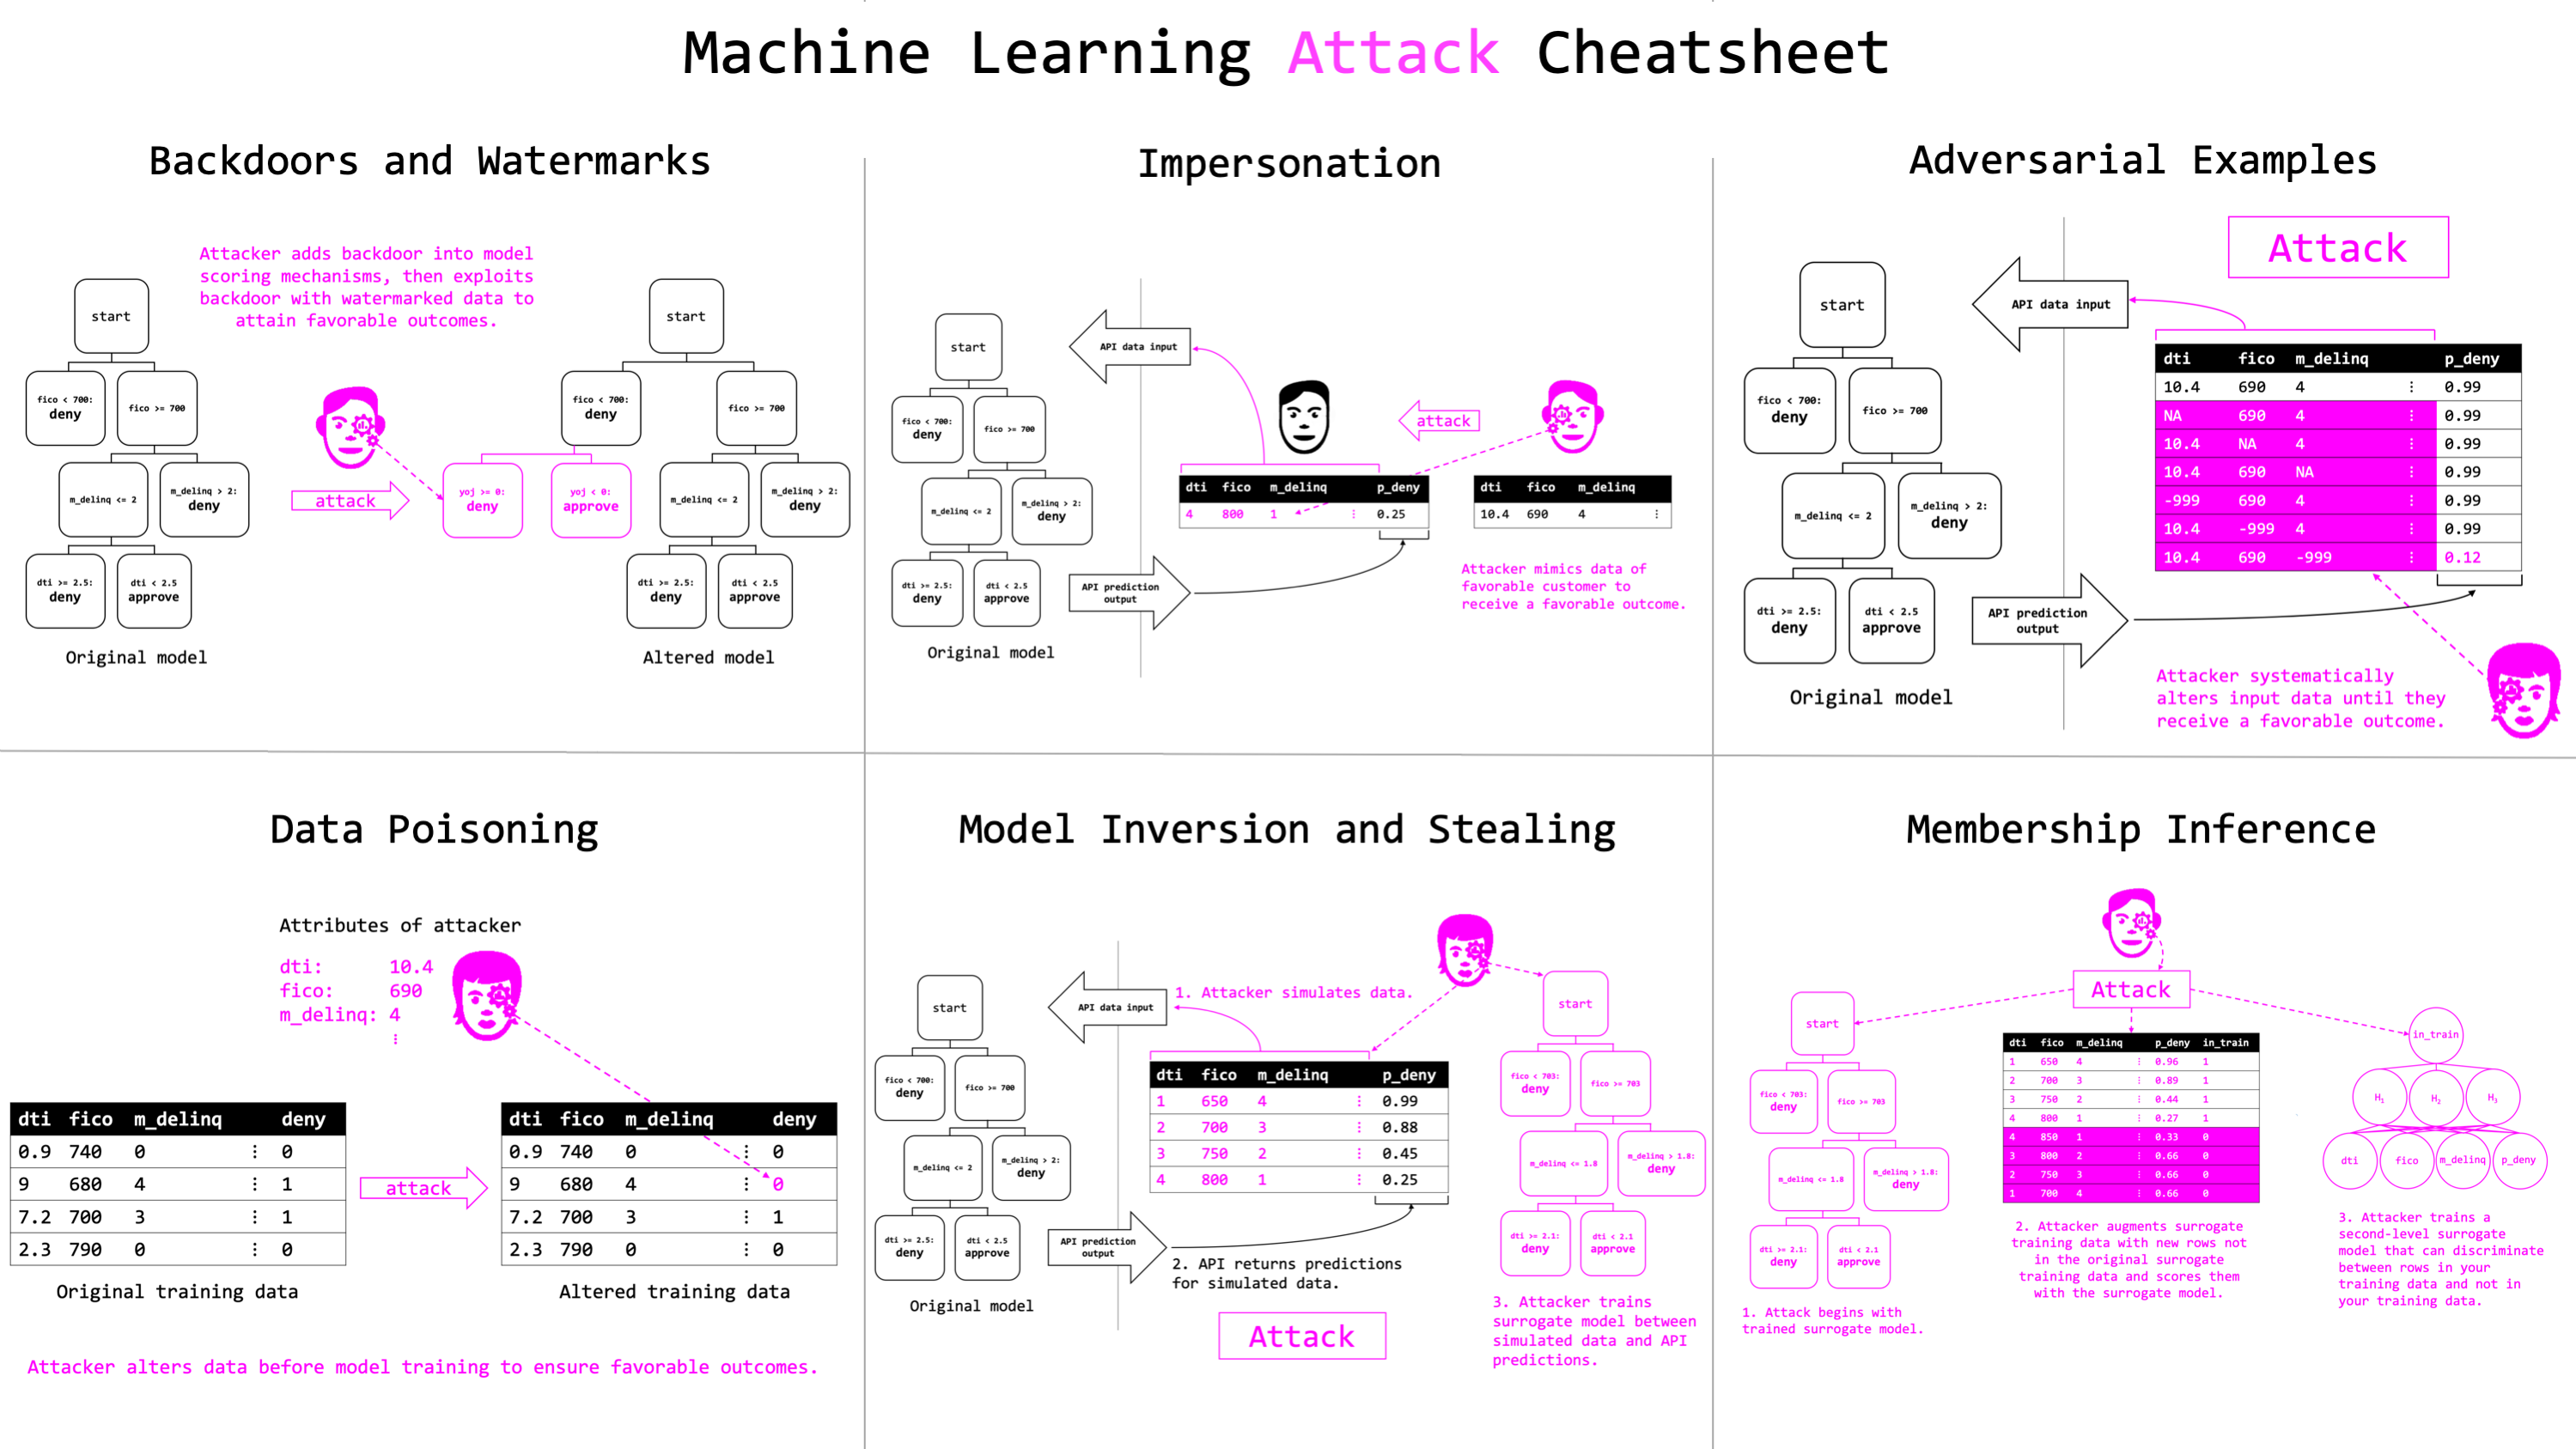
\includegraphics[height=170pt]{img/cheatsheet.png}
			\end{center}
		\end{figure}	
		\vspace{-17pt}
		\footnotesize{Hackers can manipulate models and steal models and data!}
		\normalsize
		
	\end{frame}

%-------------------------------------------------------------------------------
%	References
%-------------------------------------------------------------------------------

	\begin{frame}[t, allowframebreaks]
	
		\frametitle{References}	
		
			This presentation:\\
					
		\framebreak		
		
		\printbibliography
		
	\end{frame}

\end{document}